
\documentclass[a4paper]{article}

\usepackage[T1]{fontenc}
\usepackage[utf8]{inputenc}
\usepackage[italian]{babel}
\usepackage{listings}
\usepackage{xcolor}
\usepackage{makecell}
\usepackage{graphicx}
\usepackage{caption}
\usepackage{hyperref}
\usepackage{graphicx}
\usepackage{svg}

\usepackage{fixltx2e}


\graphicspath{{images/}}
\definecolor{darkgreen}{rgb}{0, 0.7, 0}
\lstdefinestyle{CStyle}{
	backgroundcolor =\color{white},
	commentstyle=\color{darkgreen},
	keywordstyle=\color{magenta},
	numberstyle=\tiny\color{gray},
	stringstyle=\color{mPurple},	
	basicstyle=\footnotesize,
	breakatwhitespace=false,
	breaklines=true,
	captionpos=b,
	keepspaces=true,
	numbers=left,
	numbersep=5pt,
	showspaces=false,
	showstringspaces=false,
	showtabs=false,
	tabsize=2,
	language=C	
}


\begin{document}
	
	\author{Boracchi Giacomo \and Antonio Miele \and Carrera Diego\and \\ Fioravanti Massimo}
	\title{Progetto Ingegneria Informatica \\ Datastream Change Detection}
	\maketitle
	\tableofcontents
	\clearpage
	
	\section{introduzione}


\subsection{Descrizione del problema}
\paragraph{Test di ipotesi}
Varie branche scientifiche e economiche moderne, come ad esempio la diagnostica medica, si basano sulla capacità di discernere le differenze tra popolazioni di oggetti. Se si riesce a descrivere ciò che si sta analizzando tramite variabili numeriche allora ne consegue che si sta affrontando un problema di natura matematica.
Le procedure che permettono di operare tali distinzioni sono dette test di verifica di ipotesi e la loro formulazione rigorosa giace nel dominio della statistica.
Talvolta il costo computazionale necessario per risolvere tali operazioni è assai elevato, in particolare perché la complessità degli algoritmi è spesso legata alla dimensione del campione. Inoltre se si tenta di analizzare un evento periodico reale che avviene ad alta frequenza è importante riuscire a garantire la maggiore velocità di analisi possibile, poiché ciò permette di estendere l'uso dei test di ipotesi a nuovi ambiti.
Per queste ragione è interessante studiare implementazioni efficienti dei test statistici.

\paragraph{Permutation Test}
Tal volta è possibile porre delle assunzioni riguardo quali sono i parametri delle popolazioni che si vuole studiare, in tali casi è spesso possibile creare dei test specifici particolarmente potenti. Tali test prendono il nome di test parametrici.
Altre volte le caratteristiche delle popolazioni sono completamente ignote, poiché magari derivano da eventi naturali. I test ideati per lavorare con queste popolazioni prendono il nome di test non parametrici. 
I test di permutazione sono particolari all'interno di questa categoria perché il loro funzionamento si basa sul calcolare una statistica riguardanti le popolazioni che si intende confrontare, per poi permutare casualmente i due gruppi e ripetere il calcolo. Si itera questa procedura sino ad aver raccolto dati a sufficienza, e si confronta la statistica della popolazione originale contro una soglia calcolata dalle statistiche delle permutazioni permutate. Se il primo numero risulta essere maggiore del secondo allora ne consegue che le due popolazioni non possono disporre delle stesse caratteristiche, poiché se quello fosse stato il caso allora non si discosterebbe così tanto dal caso medio ottenuto dalle permutazioni.

\paragraph{Schede Grafiche}
Gli ultimi 15 anni hanno visto l'affermarsi della tecnologia delle schede grafiche come strumento utile alla computazione ad alta velocità.
Progettate inizialmente per la creazione di immagini 3D da presentare a schermo, tali unità di calcolo presentano caratteristiche che le rendono adatte a eseguire calcoli in parallelo.
Una scheda grafica è composta svariate unità di calcolo ognuna disposta dei propri registri privati, queste unità sono poi raggruppate a gruppi i quali condividono una memoria locale e infine tutte loro accedono alla stessa memoria globale. 
I gruppi condividono anche parte delle componenti hardware, in particolare quelle legate al controllo del flusso del programma. Ciò implica che mentre il consumo energetico è minore rispetto alle cpu convenzionali, le unità di calcolo all'interno di un gruppo devono necessariamente eseguire le stesse operazioni. Tale tecnica prende il nome di SIMD, cioè Single Instruction Multiple Data, poiché disponendo di registri diversi per ogni nucleo di calcolo è possibile raggiungere risultati distinti su ognuno di essi, anche se la procedura è la stessa.

Tale architettura permette quindi di accelerare tutti gli algoritmi che possono essere eseguiti in parallelo. Se si seleziona una statistica adatta, questo è esattamente il caso riguardante i permutation test, poiché le permutazione non necessitano di conoscere quale fosse stato il risultato della permutazione precedente, mentre i calcolo della statistica segue le stesse operazioni in ogni unità di calcolo.

\paragraph{Risultati}
In questo documento si presenterà una soluzione software del problema sopra descritto destinata all'uso su schede grafiche dotata delle seguenti caratteristiche:
\begin{itemize}
	\item \textbf{Test multivariati} l'analisi di campioni multidimensionali risulta particolarmente difficile e costosa, la nostra implementazione risolve tale problema per costruzione.
	\item \textbf{Memoria lineare} il nostro algoritmo richiede memoria pari a quella necessaria per allocare l'input in ingresso. Tale soluzione è ideale poiché la memoria disponibile sulle schede grafiche è limitata e garantire tale proprietà nel problema affrontato è difficile.
	\item \textbf{Accesso sequenziale} il nostro algoritmo accede alla memoria in maniera sequenziale ed esattamente una volta per ogni elemento, tale soluzione è ideale poiché l'accesso non ordinato rallenta significativamente l'efficienza delle schede grafiche.
\end{itemize}

	\section{Fondamenti teorici}


\subsection{Statistica}
Definiamo come statistica una funzione che associa a una popolazione un numero reale che la rappresenta. Ad esempio la funzione che associa ad una popolazione di lunghezze la media di tali valori è una statistica.
 

\subsection{Test di ipotesi}
Per test di verifica di ipotesi si intende un test ideato per verificare su un ipotesi risulta essere vera o meno, e per ipotesi si intende un affermazione riguardante oggetti del mondo reale. I test di ipotesi di dividono in test di ipotesi deterministici o statistici, ed è su questi ultimi che ci concentreremo.

L'ipotesi da verificare prende il nome di H\textsubscript{0} o ipotesi nulla. Si definisce invece l'ipotesi contraria come H\textsubscript{1} o ipotesi alternativa.
Come conseguenza di un test vi possono essere due tipi di errori, rifiutare l'ipotesi nulla quando essa era vera, come ad esempio non identificare una malattia in un paziente malato, oppure accettare l'ipotesi nulla quando essa è falsa, ad esempio identificare una malattia in un paziente sano. Il primo caso prende il nome di errore di primo caso, e il secondo errore di secondo tipo.
Minimizzare gli errori del primo tipo senza curarsi degli errori del secondo è triviale, poiché è sufficiente accettare ogni volta l'ipotesi. Similarmente è vero l'inverso, rifiutare sempre l'ipotesi H\textsubscript{0} permette di minimizzare gli errori del secondo tipo ma garantisce di massimizzare quelli del primo.
Di conseguenza la maniera corretta di formulare un test é garantire costanti gli errori del primo tipo, ad esempio il 5\% dei casi, e si desidera minimizzare gli errori del secondo tipo. La soglia mantenuta costante è detta $\alpha$.
Il valore calcolato come 1 meno errori del secondo tipo è detto potenza del test.

Come conseguenza del fatto che gli errori del primo tipo devono essere costanti ne consegue che per certe statistiche è possibile calcolare dei valori di soglia che quando confrontati con la statistica valutata per una popolazione che rispetta l'ipotesi h\textsubscript{0} soddisfano la richiesta che gli errori del primo tipo siano esattamente $\alpha$\%.
Questi valori, detti soglie, sono poi utilizzati come di valori di confronto nel caso di popolazioni che si vuole determinare se soddisfano l'ipotesi nulla o meno, e in questa maniera si può ricavare una procedura algoritmica che permetta di eseguire il test di ipotesi.

\subparagraph{Permutation Test}
In alcuni casi le soglie dipendono dalla struttura dei dati in ingresso, in particolare quando i dati hanno una natura vettoriale, e di conseguenza non è possibile calcolarle in anticipo. In tali situazioni è necessario affidarsi ad altre soluzioni e una di queste è il permutation test che permette di stabilire se due gruppi provengono dalla stessa popolazione. La considerazione sulla quale si basa un permutation test è che se si permutano i due gruppi casualmente allora in media $\alpha$ \% delle volte la statistica calcolata avrà un valore maggiore della soglia ignota, poiché permutando il campione allora sarà impossibile distinguere gli elementi appartenenti al primo gruppo da quelli appartenenti al secondo. 
Se si ordinano le statistiche valutate sulle popolazioni permutate e si seleziona quella nella posizione numero permutazioni * (1-$\alpha$). Tale valore risulta essere una stima della soglia, ed è quindi possibile eseguire test di ipotesi statistica pur essendo del tutto ignari della distribuzione di una popolazione.
	
	\section{Implementazione}

\subsection{Implementazione C} \label{impC}
L'algoritmo è composto da due fasi, il calcolo delle statistiche per ogni permutazione e il confronto dei risultati ottenuti.
Poiché il risultato deve essere un booleano che indica se le popolazioni dispongono delle stesse caratteristiche, e la statistica è indipendente dal test allora ne consegue la intestazione della stringa c può essere la seguente


\begin{lstlisting}[style=CStyle]
int runPermutationTest(Data *data, float (*statistic)(Data* data));
\end{lstlisting}

Data è la struct contenente è definita come segue

\begin{lstlisting}[style=CStyle]

typedef struct data
{	
	float* sample;
	unsigned size;
	unsigned cutPoint;
	float alpha;
	float iterations;
} Data;

\end{lstlisting}

dove sample è il puntatore al primo elemento dell'array dei dati che include entrambe le popolazioni, cutPoint è la dimensione della prima popolazione (e di conseguenza l'indice del primo elemento della seconda) e size è la somma della dimensione del primo campione e del secondo. La dimensione del secondo campione può essere ricavata come size - cutPoint. Alpha è il livello di significatività del test, mentre iterations è il numero di iterazioni da effettuare.

Si noti anche il secondo parametro
\begin{lstlisting}[style=CStyle]
float (*statistic)(Data* data)
\end{lstlisting}

tale scrittura indica che il secondo parametro è una funzione che accetta un puntatore a Data e ritorna un float, cioè una funzione che rappresenta una statistica.

La funzione diventa trivialmente.

\begin{lstlisting}[style=CStyle]

int runPermutationTest(Data *data, float (*statistic)(Data* data))
{
	float statistics[data->iterationsCount];
	
	//calcolo della statistica delle popolazioni non permutate
	float sampleStatistic = statistic(data); 	
	
	//calcolo delle statistiche permutate
	for (unsigned a = 0; a < data->iterations; a++)
	{
		permutate(data);
		statistics[a] = statistic(data);
	}
	
	//confronto della statistica con quelle permutate
	sort(statistics, data->iterations, sizeof(float));
	int k = data->iterations-((int)(data->alpha * data->iterations));	
	return statistics[k] > sampleStatistic;
	
}
\end{lstlisting}

La parte in cui si gestisce il caso statistics[k] == sampleStatistic del return è stato ignorato in favore della semplicità della descrizione. In tali situazioni è sufficiente generare un numero casuale tra 0 e 1 e accettare il risultato se tale valore è inferiore ad alpha. Ciò garantisce che anche nel caso si esegua una permutazione sola il numero di falsi allarmi sarà esattamente alpha.


\paragraph{OpenCL}

Gli ultimi 15 anni hanno visto l'affermarsi della tecnologia delle schede grafiche come strumento utile alla computazione ad alta velocità.
Progettate inizialmente per la creazione di immagini 3D da presentare a schermo, tali unità di calcolo presentano caratteristiche che le rendono adatte a eseguire calcoli in parallelo.
Una scheda grafica è composta svariate unità di calcolo ognuna disposta dei propri registri privati, queste unità sono poi riunite in gruppi i quali condividono una memoria locale e infine tutte loro accedono alla stessa memoria globale. 
I gruppi condividono anche parte delle componenti hardware, in particolare quelle legate al controllo del flusso del programma. Ciò implica che mentre il consumo energetico è minore rispetto alle cpu convenzionali, le unità di calcolo all'interno di un gruppo devono necessariamente eseguire le stesse operazioni. Tale tecnica prende il nome di SIMD, cioè Single Instruction Multiple Data, poiché disponendo di registri diversi per ogni nucleo di calcolo è possibile raggiungere risultati distinti su ognuno di essi, anche se la procedura è la stessa.

Tale architettura permette quindi di accelerare tutti gli algoritmi che possono essere eseguiti in parallelo. Questo è esattamente il caso riguardante i permutation test, se si seleziona una statistica adatta, poiché le permutazione non necessitano di conoscere quale fosse stato il risultato della permutazione precedente, mentre i calcolo della statistica segue le stesse operazioni in ogni unità di calcolo.

Si è mostrato come l'implementazione in un linguaggio di programmazione regolare risulta essere triviale, discuteremo ora di come implementare tale algoritmo in OpenCL, cioè uno dei linguaggi utilizzati dalle schede grafiche. Un programma OpenCL prende il nome di kernel. Un kernel è fondamentalmente una funzione che viene invocata da un normale programma risiedente nella macchina ospite della scheda. L'invocatore deve specificare quali sono i parametri di invocazione, e quale è l'area memoria dove il kernel può scrivere il risultato computato. 
Inoltre è necessario specificare quante unità di calcolo vogliamo dedicare all'operazione, anche se tale valore non è accessibile all'interno di un programma OpenCl.

Ad esempio supponiamo di voler scrivere un kernel che raddoppia il valore di ogni elemento di un array


\begin{lstlisting}[style=CStyle]
__kernel void double(__global const float *in, __global float *out)
{
	unsigned int i = get_global_id(0);
	
	out[i] = in[i] * 2;
}
\end{lstlisting}

Il programma invocante caricherà nel vettore in i dati da raddoppiare, creerà l'array out dal quale desidera ricavare i risultati e infine lancerà il kernel, indicando che desidera dedicare un numero di core pari alla dimensione dell'array.

Ogni core utilizzerà la funzione get\_global\_id per ricavare il proprio offset rispetto alla prima unità di calcolo e utilizzerà questo valore per scoprire quale numero deve raddoppiare e dove deve essere salvato.

La keyword \_\_global serve per indicare alla scheda che è un riferimento alla memoria condivisa tra tutte le unità di calcolo. 

\subparagraph{Implementazione permutation test}
Risulta triviale identificare quale parti dell'implementazione descritta nella sezione \ref{impC} sono adatti ad essere selezionati per essere svolti in parallelo.

I dati originali vengono ospitati sulla scheda, il ciclo contenuto del ciclo for viene spostato, nel kernel che si desidera scrivere, mentre l'ordinamento e il confronto vengono operati sulla cpu.


Risulta quindi che un kernel è composto dalla permutazione e dalla valutazione della statistica. 

\begin{lstlisting}[style=CStyle]
	__kernel void p_test
	(
	__global const float* in,
	__global float* out,
	unsigned int cutPoint,
	unsigned int sampleSize,
	)
	{
		unsigned int i = get_global_id(0);
		float[sampleSize] permutated;
		
		permutate(in, permutated, i);
		
		b[i] = evaluateStatistic(in, sampleSize, cutPoint, vectorSize);
	}
\end{lstlisting}

La scrittura efficiente della statistica verrà analizzata nella sezione \ref{ottimizzazione}, e
L'intero problema si riduce alla capacità di permutare i dati in ingresso.

Ciò è possibile basandosi sulla seguente osservazione:
Sia P un numero primo qualsiasi, allora $$ \forall X, Y  \in [0, P/ 2]  X \neq Y \Rightarrow (X * X) \% P \neq (Y * Y) \% P.$$
Ciò significa che iterando attraverso tutti i numeri minori di P è possibile ottenere una sequenza di numeri che non si ripetono mai.
 
\begin{lstlisting}[style=CStyle]
unsigned int singlePermutate(unsigned int x, unsigned int prime)
{	
	if (x <= prime / 2)
		return x * x % prime;
	else
		return prime - (x * x % prime);	

}
\end{lstlisting}

Si noti che alcune ottimizzazioni sono necessarie per rompere la simmetria centrale dovuta al funzionamento della formula, ma verranno tralasciate per semplicità.

Da questa funzione segue che la variabile X rappresenta il seme del generatore di numeri casuali, e quindi è sufficiente a rappresentarne completamente lo stato. 

Il kernel diviene quindi, a patto che sample size sia uguale un numero primo .
\begin{lstlisting}[style=CStyle]
	__kernel void p_test
	(
	__global const float* in,
	__global float* out,
	unsigned int cutPoint,
	unsigned int sampleSize,
	)
	{
		unsigned int i = get_global_id(0);
		float[sampleSize] permutated;
		
		for (int a = 0; a < sampleSize; a++)
			permutated[i] =int[singlePermutate(a, sampleSize)];
		
		b[i] = evaluateStatistic(in, sampleSize, cutPoint, vectorSize);
	}
\end{lstlisting}

Risulta quindi che tutto ciò che rimane da fare è ordinare i risultati e confrontarli con la statistica dei dati non premutati. Ciò può svolto dal programma risiedente nella memoria principale della macchina, poiché è necessario attendere che tutte le statistiche vengano valutate e nel caso si utilizzasse più di una scheda non vi è alcuna garanzia che esse terminino in contemporanea. 


\subsection{Test Multivariati}
Queste ottimizzazioni riguardano esclusivamente la maniera in cui si accede ai dati depositati nella memoria della scheda. Di conseguenza è possibile caricare dati sotto forma di struct, invece che semplici float. Risulta quindi raggiunto uno degli obiettivi di tale documento, disponiamo di un implementazione di un test di ipotesi capace di operare su campioni multivariati che non necessita di precalcolare le soglie.
	\section{Ottimizzazione} \label{ottimizzazione}

\subsection{Permutazioni a spazio costante e visita ordinata}
Poiché le computazioni avvengono in parallelo, non è possibile permutare sul posto i dati in ingresso, poiché ciò richiederebbe una quantità di memoria pari alla dimensione dei dati in ingresso moltiplicati per il numero di permutazioni, poiché ogni unità di calcolo deve allocare localmente i dati permutati. Risulta quindi imperativo utilizzare un algoritmo a spazio costante, poiché la memoria disponibile per ogni singolo core è limitata.
Si mostrerà ora come è possibile computare statistiche che operano in maniera sequenziale senza precalcolare la permutazione da applicare ai dati.

Prendiamo come esempio la statistica che date due popolazioni ritorna la differenza delle loro medie.

\begin{lstlisting}[style=CStyle]
float evaluateStatistic
(
	__global const float* in, 
	const unsigned int sampleSize, 
	const unsigned int cutPoint
)
{
	float meanSample1 = 0;
	float meanSample2 = 0;
	
	for (int a = 0; a < cutPoint; a++)
		meanSample1 += in[a];
	meanSampel1 /= cutPoint;
		
	for (int a = cutPoint < sampleSize; a++)
		meanSample2 += in[a];
	meanSample2 /= sampleSize - cutPoint;	
	
	return abs(meanSample1 - meanSample2);
}
\end{lstlisting}

grazie alla funzione di permutazione possiamo mappare gli indici sequenziali al loro equivalente permutato, così facendo perdiamo però la possibilità di capire se l'elemento appartiene al primo gruppo o al secondo.
La funzione deve quindi essere modificata in:

\begin{lstlisting}[style=CStyle]
	float evaluateStatistic
	(
	__global const float* in,
	int prime,
	int index,
	const unsigned int sampleSize, 
	const unsigned int cutPoint
	)
	{
		float meanSample1 = 0;
		float meanSample2 = 0;
		
		for (int a = 0; a < sampleSize; a++)
		{
			int realIndex = permutateSingle(index++, prime);
			
			if (realIndex < cutPoint)
				meanSample1 += in[realIndex];
			else
				meanSample2 += in[realIndex];
		}
		
		meanSampel1 /= cutPoint;
		meanSample2 /= sampleSize - cutPoint;	
		
		return abs(meanSample1 - meanSample2);
	}
\end{lstlisting}


Si noti che questo algoritmo dispone di un altra caratteristica, l'accesso alla memoria è sequenziale e tutti i nuclei accedono contemporaneamente allo stesso elemento. Poiché le memorie globali delle schede grafiche sono molto più lente che le memorie private, questa soluzione migliora sensibilmente le performance dell'algoritmo.

\subsection{Campioni di dimensione qualsiasi}
Come precedentemente indicato, la natura del generatore di numeri casuali impone l'uso di campioni la cui dimensione è un numero primo. Tale restrizione è particolarmente insoddisfacente, quindi si discuterà ora di come rimuoverla:
Se la dimensione del campione è troppo distante da un numero primo è possibile allocare come variabile locale un array la cui dimensione è pari alla differenza tra la dimensione e il minimo primo maggiore della dimensione stessa. Ogni volta che si estrae dalla permutazione un numero maggiore della dimensione del campione si salva il valore proveniente dall'array di input nell'array locale in maniera sequenziale. Dopo aver processato tutti gli elementi dell'array globale si processano nuovamente tutti quelli allocati localmente, con la garanzia che ora l'indice estratto sarà minore della dimensione del campione, poiché tutti gli indici maggiori sono già stati valutati.


\begin{lstlisting}[style=CStyle]
float evaluateStatistic
(
__global const float* in,
int prime,
int index,
const unsigned int sampleSize, 
const unsigned int cutPoint
)
{
	float meanSample1 = 0;
	float meanSample2 = 0;
	float[prime - sampleSize] local;
	int lastAllocatedIndex = 0;
	
	
	for (int a = 0; a < sampleSize; a++)
	{
	
		int realIndex = permutateSingle(index++, prime);
		if (realIndex > sampleSize)
			local[lastAllocatedIndex++] = in[realIndex];
		else if (realIndex < cutPoint)
			meanSample1 += in[realIndex];
		else
			meanSample2 += in[realIndex];
	}
	
	for (int a = 0; a < prime - sampleSize; a++)
	{
		int realIndex = permutateSingle(index++, prime);
		
		if (realIndex > sampleSize)
			local[lastAllocatedIndex++] = local[realIndex];
		else if (realIndex < cutPoint)
			meanSample1 += local[realIndex];	
		else
			meanSample2 += local[realIndex];
	}
	
	meanSampel1 /= cutPoint;
	meanSample2 /= sampleSize - cutPoint;	
	
	return abs(meanSample1 - meanSample2);
}
\end{lstlisting}


Disponiamo quindi di un algoritmo che accede in maniera sequenziale a tutti gli elementi in memoria ed è capace di permutarli in parallelo utilizzando una quantità di memoria, oltre a quella richiesta dallo spazio dedicato all'input e all'output, costante.
	\section{Analisi e Conclusioni}

\subsection{Controllo dei falsi allarmi}
La correttezza dell'implementazione di un test di ipotesi può essere controllata assicurandosi che in condizioni di ipotesi nulla il test produca esattamente $\alpha$\% falsi allarmi. Il test deve poi presentare la maggiore potenza possibile in caso di ipotesi contraria. Per utilizzare una metrica di riferimento abbiamo utilizzato i test inclusi nella libreria standard di matlab.
Mostriamo quindi il risultati ottenuti dall'uso di una semplice statistica, la differenza delle medie:

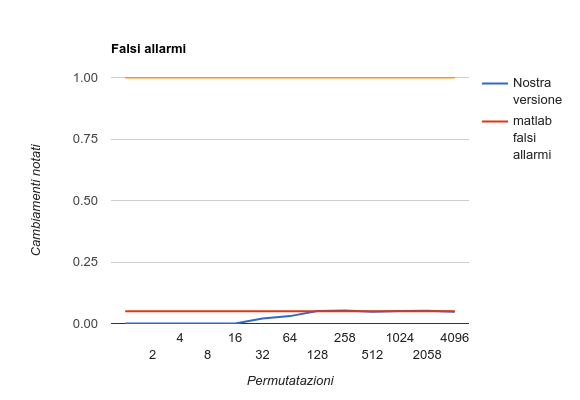
\includegraphics[width=\linewidth]{falsi_allarmi}

La linea rossa è generata da matlab non dipende dal numero di permutazioni, quindi è costante a 0.05, come ci si attende. La linea blu rappresenta invece la nostra versione del permutation test, la quale per bassi valori di permutazione è del tutto incapace di notare cambiamenti nei valori in ingresso. Quando le permutazioni aumentano i falsi allarmi si stabilizzano velocemente ad $\alpha$. 

Ora che siamo certi che sotto ipotesi nulla il nostro algoritmo si comporta correttamente, possiamo quindi analizzare il caso in cui i gruppi provengono da popolazioni diverse.

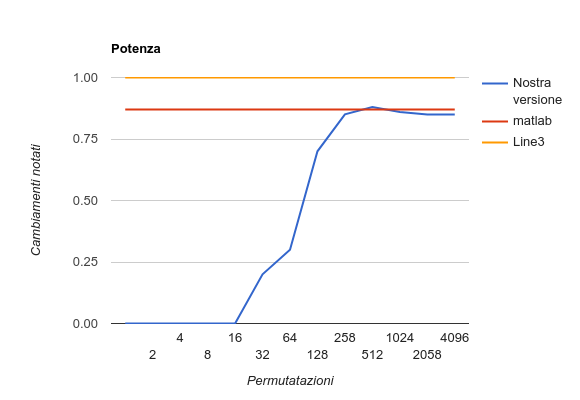
\includegraphics[width=\linewidth]{potenza}

Come nel caso precedente si nota che pur fallendo per permutazioni in quantità minute risulta che il test produce risultati simili a quello standard. Si noti inoltre che come nel caso precedente non sembra esserci alcun vantaggio nell'utilizzare un grande numero di permutazioni, poiché quando raggiungono l'ordine delle centinaia la potenza si stabilizza. Questo significa che, date le ottimizzazioni sull'uso della memoria, se si fissa un numero di permutazioni, è possibile processare set di dati con utilizzi di tempo e memoria che dipendono linearmente solo dalla dimensione dei dati in ingresso. Poiché è evidente che per processare un set di dati è per lo meno necessario valutare almeno una volta tutti gli elementi, ciò risulta essere il migliore risultato possibile. 

Ciò che rimane è mostrare la velocità di throughput che è possibile raggiungere è superiore ad un implementazione basata su cpu.

\subsection{Benchmark}

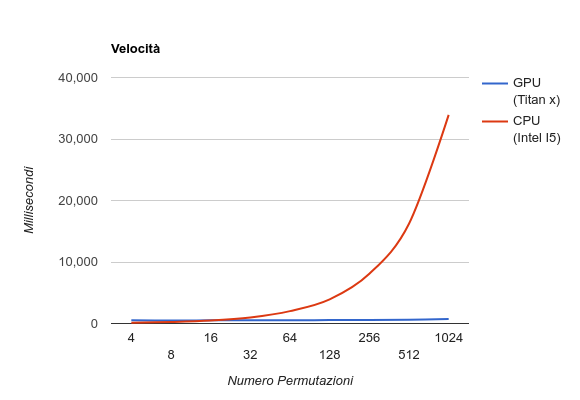
\includegraphics[width=\linewidth]{confronto}

Il tempo necessario al completamento del calcolo dell'implementazione su cpu dipende linearmente dalla quantità di permutazioni, e allo spostarsi verso destra sull'asse X diventa rapidamente troppo lento. La implementazione GPU invece sembra rimanere a tempo costante, ciò è dovuto al fatto che le permutazioni non superano in quantità il numero di core a disposizione sulla scheda e quindi tutti il calcoli possono avvenire allo stesso momento. 
Come ci si aspettava l'implementazione su GPU risulta essere meno performante per piccoli valori di permutazioni, dove i vantaggi dell'architettura parallela sono ridotti, ma non appena si supera una soglia critica la implementazione su gpu risulta più efficiente sotto tutti gli aspetti.

Studiano più accuratamente solo i risultati della gpu risulta inoltre:

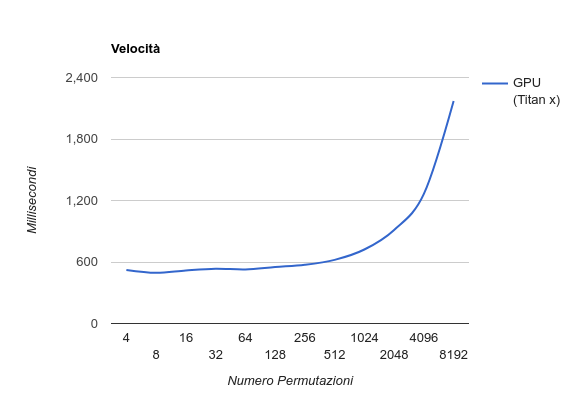
\includegraphics[width=\linewidth]{analisi}

Per piccoli valori di permutazioni il tempo richiesto è effettivamente costante, mentre esso ritorna a dipendere linearmente dal numero di permutazioni non appena la scheda viene saturata.
Anche in questo caso il tempo per impiegare 8192 permutazioni è circa 2.5, inferiore a quello necessario per compierne 512 su una cpu. Si noti inoltre che non si erano trovati significativi incrementi di potenza quando il numero di permutazioni superava l'ordine delle centinaia, di conseguenza non vi è motivo di operare nello spazio in cui il tempo di esecuzione dipende linearmente dal numero di permutazioni. Ciò trasforma la nostra implementazione in un algoritmo che opera a tempo costante su set di dati di dimensione fissata dotato di potenza simile a quella dei test disponibili nelle librerie standard ma con un througthput maggiore e capace di operare su dati multivariati, il che era l'obiettivo che si intendeva raggiungere in questo documento.

Le ottimizzazioni inoltre producono i seguenti incrementi in performance:
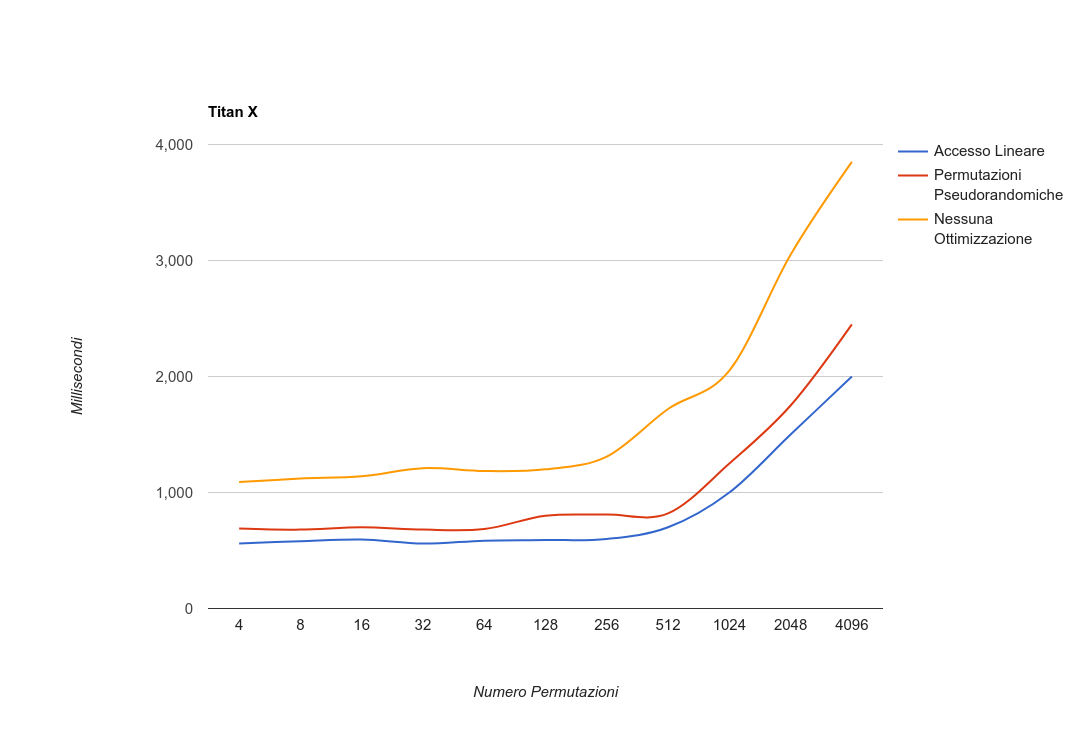
\includegraphics[width=\linewidth]{ott}

La linea blu rappresenta l'implementazione opencl triviale, come ci si aspetta risulta essere due volte peggiore che la implementazione ottimizzata. La linea rossa rappresenta invece la versione dell'algoritmo dotata di permutazione pseudorandomica ma di cui non è garantito l'accesso ordinato alla memoria. In questo caso ne prestazioni sono paragonabili alle migliori rilevate, sebbene una diminuzione del tempo di calcolo di un sesto giustifica l'uso di codice più complesso e difficile da mantenere.

\subsection{Lavori Futuri}
A seconda di quale sia il campo di applicazione di un test di ipotesi ad alta performanza è possibile che ulteriori caratteristiche oltre a quelle indicare siano richieste. Si può immaginare che la necessità di analizzare eventi che avvengono ad alta frequenza sia spesso associata alla necessità di processare tali dati sotto forma di stream continui fino a che non viene notato un cambiamento nella natura dei dati osservati.
Una delle soluzioni di tale problema prende il nome di Change Point Model (CPM) e consiste nell'analizzare i dati per ogni possibile posizione del change point, per poi selezionare la posizione che più si è discostata dalla soglia. Il tentativo di integrare efficientemente il permutation test e il cpm si è rivelato inconcludente. Inoltre, anche le integrazioni più semplici sono inefficienti, poiché le ottimizzazioni necessarie ad uno risultano deleterie all'altro. Questo limite pare significativo e ne consegue che la risoluzione possa essere soggetto di ulteriori studi.
\end{document}